% This file has been generated automatically by teachmedijkstra 0.1.0
% Time of the creation: 2022-05-16 19:31:37.700483

% teachmedijkstra is a Python3 package
% web page: https://gitlab.com/petrikm/teachmedijkstra
% author: Milan Petrík
% e-mail: milan.petrik@protonmail.com

\documentclass{article}

% Import TikZ to draw the graph and the shortest path tree
\usepackage{tikz}
% TikZ library to depict the edges of a directed graph as arrows
\usetikzlibrary{arrows}
% To have a clickable reference to the web page of teachmedijkstra
\usepackage{hyperref}

\begin{document}

\begin{center}
    {\LARGE Dijkstra's algorithm\footnote{
    This document has been generated automatically by \texttt{teachmedijkstra-0.1.0}
    which is a Python3 package
    available at \url{https://gitlab.com/petrikm/teachmedijkstra}.
    }}
\end{center}

\begin{center}
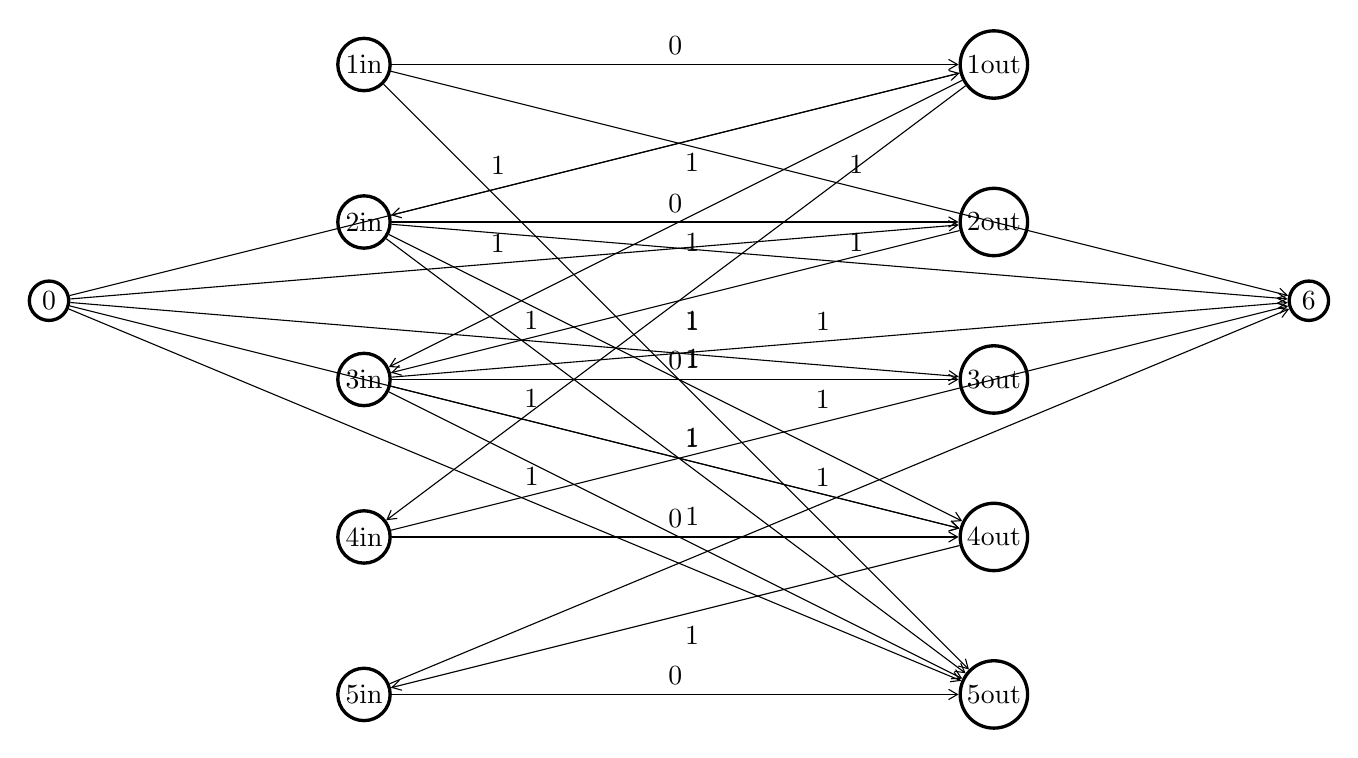
\begin{tikzpicture}[scale=2, auto]
    \tikzstyle{graph vertex} = [circle,draw=black,fill=white,very thick,inner sep=1.5pt, minimum size=5mm]
    \tikzstyle{graph edge undirected} = [draw=black]
    \tikzstyle{graph edge directed} = [graph edge undirected, ->, >=angle 60]
\node[graph vertex] (0) at (-4, -2.5) {0};
\node[graph vertex] (1in) at (-2, -1) {1in};
\node[graph vertex] (1out) at (2, -1) {1out};
\node[graph vertex] (2in) at (-2, -2) {2in};
\node[graph vertex] (2out) at (2, -2) {2out};
\node[graph vertex] (3in) at (-2, -3) {3in};
\node[graph vertex] (3out) at (2, -3) {3out};
\node[graph vertex] (4in) at (-2, -4) {4in};
\node[graph vertex] (4out) at (2, -4) {4out};
\node[graph vertex] (5in) at (-2, -5) {5in};
\node[graph vertex] (5out) at (2, -5) {5out};
\node[graph vertex] (6) at (4, -2.5) {6};
\draw[graph edge directed] (1in) to node {0} (1out);
\draw[graph edge directed] (1in) to node {1} (5out);
\draw[graph edge directed] (1in) to node {1} (6);
\draw[graph edge directed] (2in) to node {0} (2out);
\draw[graph edge directed] (2in) to node {1} (4out);
\draw[graph edge directed] (2in) to node {1} (5out);
\draw[graph edge directed] (2in) to node {1} (6);
\draw[graph edge directed] (3in) to node {0} (3out);
\draw[graph edge directed] (3in) to node {1} (4out);
\draw[graph edge directed] (3in) to node {1} (5out);
\draw[graph edge directed] (3in) to node {1} (6);
\draw[graph edge directed] (4in) to node {0} (4out);
\draw[graph edge directed] (4in) to node {1} (6);
\draw[graph edge directed] (5in) to node {0} (5out);
\draw[graph edge directed] (5in) to node {1} (6);
\draw[graph edge directed] (1out) to node {1} (2in);
\draw[graph edge directed] (1out) to node {1} (3in);
\draw[graph edge directed] (1out) to node {1} (4in);
\draw[graph edge directed] (2out) to node {1} (3in);
\draw[graph edge directed] (4out) to node {1} (5in);
\draw[graph edge directed] (0) to node {1} (1out);
\draw[graph edge directed] (0) to node {1} (2out);
\draw[graph edge directed] (0) to node {1} (3out);
\draw[graph edge directed] (0) to node {1} (4out);
\draw[graph edge directed] (0) to node {1} (5out);
\end{tikzpicture}
\end{center}
\begin{center}
\begin{tabular}{|r||c@{\,}c|}
\hline
 & & 1.\\
\hline
0 & $\cdot$ & 0\\
\hline
1in & $\cdot$ & $\infty$\\
\hline
1out & $\cdot$ & $\infty$\\
\hline
2in & $\cdot$ & $\infty$\\
\hline
2out & $\cdot$ & $\infty$\\
\hline
3in & $\cdot$ & $\infty$\\
\hline
3out & $\cdot$ & $\infty$\\
\hline
4in & $\cdot$ & $\infty$\\
\hline
4out & $\cdot$ & $\infty$\\
\hline
5in & $\cdot$ & $\infty$\\
\hline
5out & $\cdot$ & $\infty$\\
\hline
6 & $\cdot$ & $\infty$\\
\hline
\end{tabular}
\end{center}
\begin{center}
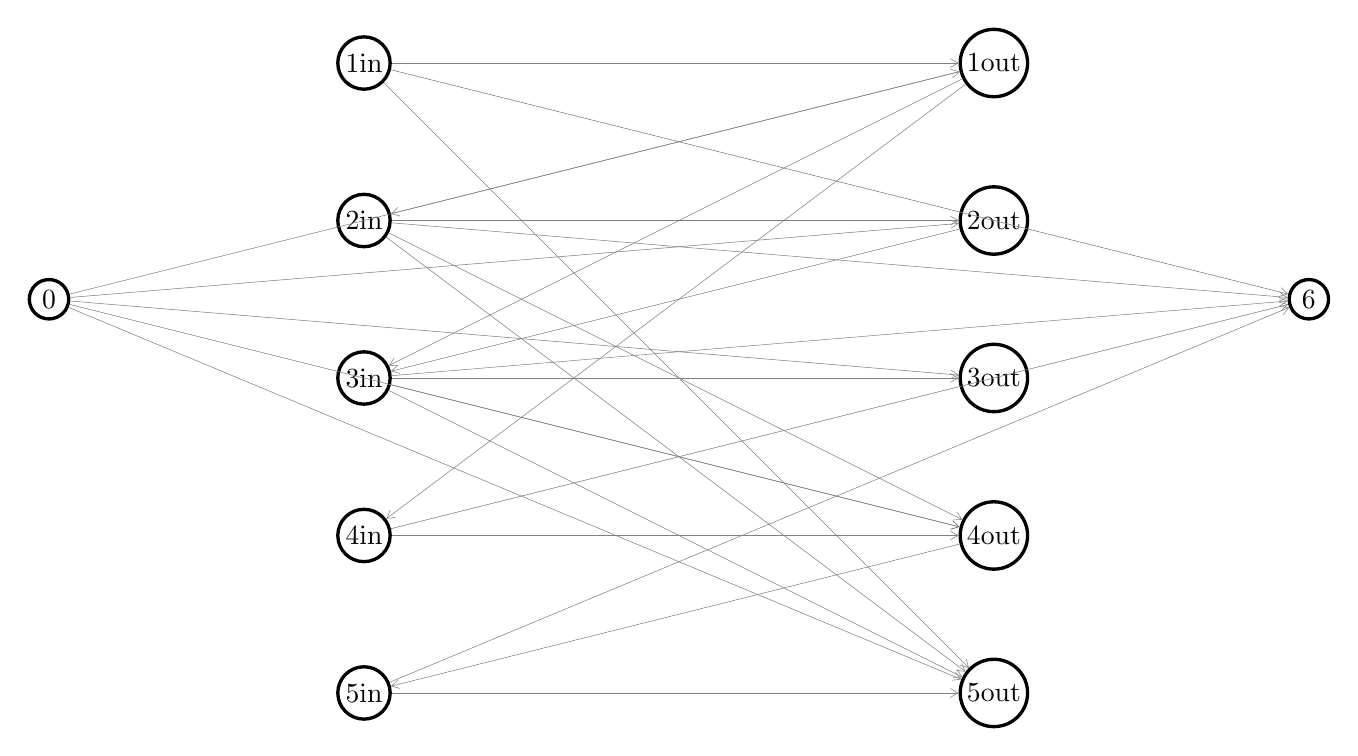
\begin{tikzpicture}[scale=2, auto]
    \tikzstyle{graph vertex} = [circle,draw=black,fill=white,very thick,inner sep=1.5pt, minimum size=5mm]
    \tikzstyle{graph edge undirected} = [draw=black]
    \tikzstyle{graph edge directed} = [graph edge undirected, ->, >=angle 60]
\node[graph vertex] (0) at (-4, -2.5) {0};
\node[graph vertex] (1in) at (-2, -1) {1in};
\node[graph vertex] (1out) at (2, -1) {1out};
\node[graph vertex] (2in) at (-2, -2) {2in};
\node[graph vertex] (2out) at (2, -2) {2out};
\node[graph vertex] (3in) at (-2, -3) {3in};
\node[graph vertex] (3out) at (2, -3) {3out};
\node[graph vertex] (4in) at (-2, -4) {4in};
\node[graph vertex] (4out) at (2, -4) {4out};
\node[graph vertex] (5in) at (-2, -5) {5in};
\node[graph vertex] (5out) at (2, -5) {5out};
\node[graph vertex] (6) at (4, -2.5) {6};
\draw[graph edge directed, very thin, gray] (1in) to (1out);
\draw[graph edge directed, very thin, gray] (1in) to (5out);
\draw[graph edge directed, very thin, gray] (1in) to (6);
\draw[graph edge directed, very thin, gray] (2in) to (2out);
\draw[graph edge directed, very thin, gray] (2in) to (4out);
\draw[graph edge directed, very thin, gray] (2in) to (5out);
\draw[graph edge directed, very thin, gray] (2in) to (6);
\draw[graph edge directed, very thin, gray] (3in) to (3out);
\draw[graph edge directed, very thin, gray] (3in) to (4out);
\draw[graph edge directed, very thin, gray] (3in) to (5out);
\draw[graph edge directed, very thin, gray] (3in) to (6);
\draw[graph edge directed, very thin, gray] (4in) to (4out);
\draw[graph edge directed, very thin, gray] (4in) to (6);
\draw[graph edge directed, very thin, gray] (5in) to (5out);
\draw[graph edge directed, very thin, gray] (5in) to (6);
\draw[graph edge directed, very thin, gray] (1out) to (2in);
\draw[graph edge directed, very thin, gray] (1out) to (3in);
\draw[graph edge directed, very thin, gray] (1out) to (4in);
\draw[graph edge directed, very thin, gray] (2out) to (3in);
\draw[graph edge directed, very thin, gray] (4out) to (5in);
\draw[graph edge directed, very thin, gray] (0) to (1out);
\draw[graph edge directed, very thin, gray] (0) to (2out);
\draw[graph edge directed, very thin, gray] (0) to (3out);
\draw[graph edge directed, very thin, gray] (0) to (4out);
\draw[graph edge directed, very thin, gray] (0) to (5out);
\end{tikzpicture}
\end{center}
\end{document}
